\chapter{Theory}
\section{Fluid mechanics in a rotating frame}
\begin{minipage}{0.49\textwidth}
    We would like to determine the mechanisms behind the generation of vorticity observed in hurricanes. Our first step will be to determine the effect of a rotating frame of reference on flow. To do so, we define an inertial frame of reference $S_I$ as well as a rotating frame of reference $S_R$ which rotates with angular velocity $\vec{\Omega}$ with respect to the inertial frame of reference. Suppose $\vec{A}$ is constant in the rotating frame of reference while $\Vec{B}(t)$ changes in the rotating frame (\ref{fig:fig1}). When looking at how both of these change in the inertial frame, we obtain:
    \begin{align*}
        \left(\frac{d\vec{A}}{dt}\right)_{I} &= \vec{\Omega}\cross\vec{A}
    \end{align*}
    As well as:
    \begin{align}
        \left(\frac{d\vec{B}}{dt}\right)_{I} &= \left(\frac{d\vec{B}}{dt}\right)_{R}+\vec{\Omega}\cross\vec{B}
        \label{rule1}
    \end{align}
    Let us define $\vec{B}=\vec{r}$, a position vector. Then, $\frac{d\vec{B}}{dt}=\vec{u}$ such that our equation above gives:
    \begin{align}
        \vec{u}_I &= \vec{u}_R+\vec{\Omega}\cross\vec{r}
        \label{rule2}
    \end{align}
\end{minipage}\hspace{0.05\textwidth}
\begin{minipage}{0.49\textwidth}
    \vspace{-2ex}
    \begin{center}
        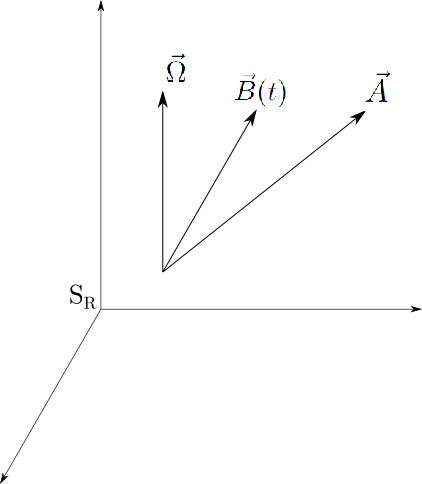
\includegraphics[width=0.9\linewidth]{assets/figure-1.png}
        \captionof{figure}{$\vec{A}$ and $\vec{\Omega}$ are constant in the rotating frame whereas $\vec{B}$ changes.}
        \label{fig:fig1}
    \end{center}
\end{minipage}

Applying \ref{rule1} to $\vec{u}_I$ gives:
\begin{align*}
    \left(\frac{d\vec{u}_I}{dt}\right)_I &= \left(\frac{d\vec{u}_I}{dt}\right)_R+\vec{\Omega}\cross\vec{u}_I
\end{align*}
Then, using \ref{rule2} gives:
\begin{align*}
    \left(\frac{d\vec{u}_I}{dt}\right)_I &= \frac{d}{dt}\left(\vec{u}_R+\vec{\Omega}\cross\vec{r}\right)_R+\vec{\Omega}\cross\left(\vec{u}_R+\vec{\Omega}\cross\vec{r}\right)_R\\
    \left(\frac{d\vec{u}_I}{dt}\right)_I &= \left(\frac{d\vec{u}_R}{dt}\right)_R+2\vec{\Omega}\cross\vec{u}_R+\vec{\Omega}\cross\left(\vec{\Omega}\cross\vec{r}\right)
\end{align*}
As per Kundu \cite{cohen2004fluid} \textit{Ch. 4, section 11}, we can define:
\begin{align*}
    \vec{\Omega}\cross\left(\vec{\Omega}\cross\vec{r}\right) &= -\vec{\nabla}\phi_c
\end{align*}
where:
\begin{align*}
    \phi_c &= \frac{\vert \vec{\Omega}\cross\vec{r}\vert^2}{2}
\end{align*}
Our equation therefore becomes:
\begin{align*}
    \vec{a}_I &= \vec{a}_R+2\vec{\Omega}\cross\vec{u}_R-\vec{\nabla}\phi_c
\end{align*}
Now, we input this in the Navier-Stokes equation:
\begin{align*}
    \rho\left(\frac{D\vec{u}_R}{Dt}+2\vec{\Omega}\cross\vec{u}_R-\vec{\nabla}\phi_c\right) &=-\vec{\nabla}p+\rho\vec{\nabla}\Phi+\mu\lap{\vec{u}_R} 
\end{align*}
If we redefine the gravitational potential as being:
\begin{align*}
    \Phi &= \phi_g+\phi_c
\end{align*}
where $\phi_g$ is the gravitational potential, we get the following modified Navier-Stokes equation for a rotating frame:
\begin{align*}
    \rho\left(\frac{D\vec{u}}{Dt}+2\vec{\Omega}\cross\vec{u}\right) &=-\vec{\nabla}p+\rho\vec{\nabla}\Phi+\mu\lap{\vec{u}} 
\end{align*}
where $\vec{u}=\vec{u}_R$. Let us then show the first of two mechanisms that generates vorticity during hurricane formation: \textit{geostrophic balance}.

\vspace{5mm}
\begin{minipage}{0.49\textwidth}
    \vspace{-2ex}
    \begin{center}
        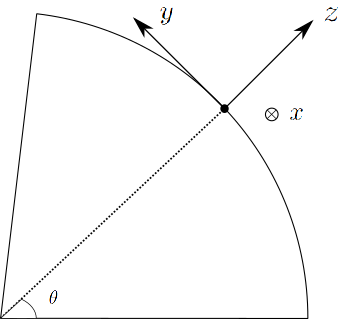
\includegraphics[width=0.7\linewidth]{assets/figure-2.png}
        \captionof{figure}{Traditional $f$-plane approximation in the Northern Hemisphere}
        \label{fig:fig2}
    \end{center}
\end{minipage}\hspace{0.05\textwidth}
\begin{minipage}{0.49\textwidth}
    Consider a small region on the surface of the Earth at latitude $\theta$ as shown by \ref{fig:fig2}. If we have this region be in a rotating frame of reference with
    \begin{align*}
        2\vec{\Omega} &= \left(0,f_h,f\right)
    \end{align*}
    where $f$ is the Coriolis parameter such that
    \begin{align*}
        f = 2\Omega\sin\theta &\qquad f_h=2\Omega\cos\theta
    \end{align*}
    defining $\vec{u}=(u,v,w)$ gives us:
    \begin{align*}
        2\vec{\Omega}\cross\vec{u} &= (0,f_h,f)\cross(u,v,w)\\
        &= (f_h w-fv,fu,f_h u)
    \end{align*}
    Let us assume that viscosity has negligible effects. We can then use each dimensions of our modified Navier-Stokes equation:
    \begin{align*}
        \rho \left(\frac{Du}{Dt}+f_hw-fv\right)&=-p_x\\
        \rho \left(\frac{Dv}{Dt}+fu\right)&=-p_y\\
        \rho\left(\frac{Dw}{Dt}+f_hu\right)&= -p_z-\rho g
    \end{align*}
\end{minipage}
This approximation for large scale flows allows us to neglect $f_h$ terms, giving
\begin{align}
    \label{eqn:mom1}
    \frac{Du}{Dt}-fv &= -\frac{1}{\rho}p_x\\
    \label{eqn:mom2}
    \frac{Dv}{Dt}+fu &= -\frac{1}{\rho}p_y\\
    \frac{Dw}{Dt} &=-p_z+\rho g
\end{align}

\section{Geostrophic flow}
We can then assume a geostrophic balance in this system, or balance between the Coriolis and pressure gradient forces:
\begin{align}
    -fv &= -\frac{p_x}{\rho}\\
    fu &= -\frac{p_y}{\rho}\\
    \label{eqn:hydrobal}
    p_z &= -\rho g
\end{align}
From these, we can identify a planar flow caused by geostrophic balance:
\begin{align*}
    \vec{u} = (u,v) &= \frac{1}{f\rho}\left(-p_y, p_x\right)
\end{align*}
We see that this planar flow follows lines perpendicular to a given pressure gradient. That is, they follow ``isobars", or lines of constant pressure, as shown by Fig. \ref{fig:fig3}.
\begin{figure}
    \centering
    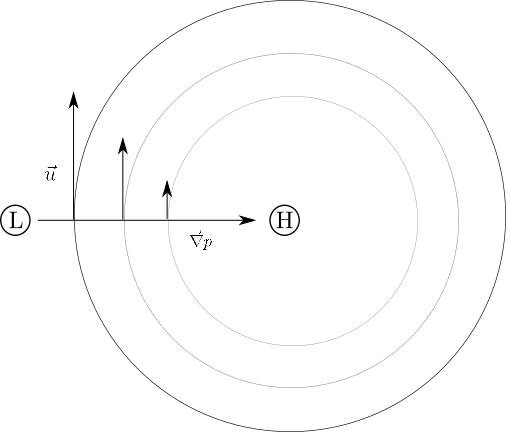
\includegraphics[width=0.5\linewidth]{assets/figure-3.png}
    \caption{Geostrophic flow is created along isobars.}
    \label{fig:fig3}
\end{figure}

When evaporation happens, high pressure appears at points where evaporation is the highest, and causes this geostrophic flow near the surface. This flow, which has other sources, is commonly referred as primary circulation. \cite{develop} 

In addition, due to conservation of angular momentum, we can show that circulation is generated when a system moves in latitude. We recall the equation for circulation:
\begin{align}
    \label{eqn:circulation}
    \Gamma (t) &= \iint_A \vec{\omega}\cdot \hat{n}dA = \oint_{\partial A} \vec{u}\cdot d\vec{r}
\end{align}
where $A$ is an area, $\partial A$ is the boundary of that area and $d\vec{r}$ is an infinitesimal piece of the boundary directed counter-clockwise. We can write our circulations for the inertial and rotating frame as
\begin{align}
    \label{eqn:incirc}
    \Gamma_I(t) &= \oint_{\partial A} \Vec{u}_I\cdot d\Vec{r}\\
    \Gamma_R(t) &= \oint_{\partial A} \Vec{u}_R\cdot d\Vec{r}\\
\end{align}
Then, recalling the relation between $\vec{u}_I$ and $\vec{u}_R$:
\begin{align}
    \label{eqn:inertrot}
    \Vec{u}_I &= \Vec{u}_R+\Vec{\Omega}\cross\Vec{r}
\end{align}
our inertial circulation becomes:
\begin{align*}
    \Gamma_I (t) &= \oint_{\partial A} (\Vec{u}_R+\Vec{\Omega}\cross\Vec{r})\cdot d\Vec{r}\\
     &= \oint_{\partial A} \Vec{u}_R\cdot d\Vec{r}+\oint_{\partial A}(\Vec{\Omega}\cross\vec
    r)\cdot d\Vec{r}\\
     &= \Gamma_R (t)+ \iint_A \Vec{\nabla}\cross(\Vec{\Omega}\cross\Vec{r})\cdot\hat{n}dA\\
     &= \Gamma_R (t) +\iint_A 2\Vec{\Omega}\cdot\hat{n}dA\\
     &= \Gamma_R (t) +2\vert \Vec{\Omega}\vert A_{\perp}
\end{align*}
where $A_{\perp}$ is the area of interest projected onto a plane perpendicular to $\Vec{\Omega}$ (in our case, a plane that goes through the equator) as demonstrated by Fig. \ref{fig:circulation}. If we take the time derivative:
\begin{align*}
    \frac{d\Gamma_I}{dt} &= \frac{d\Gamma_R}{dt}+2\vert \Vec{\Omega}\vert \frac{dA_\perp}{dt}
\end{align*}
\begin{minipage}{0.49\textwidth}
    \vspace{-2ex}
    \begin{center}
        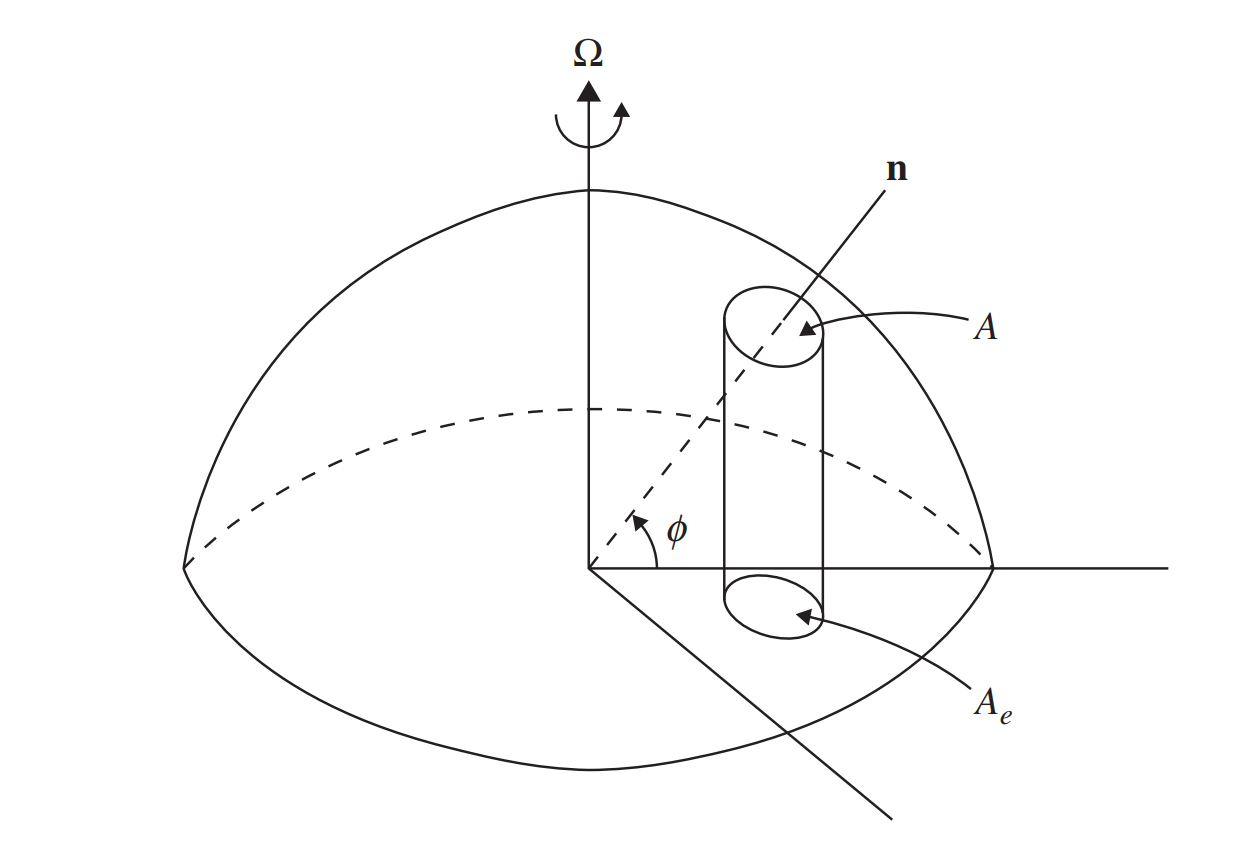
\includegraphics[width=\linewidth]{assets/circulation.png}
        \captionof{figure}{Depiction of the area of interest and it's projection onto the plane perpendicular to $\Vec{\Omega}$ from \cite{holton_hakim_2019}}
        \label{fig:circulation}
    \end{center}
\end{minipage}\hspace{0.05\textwidth}
\begin{minipage}{0.49\textwidth}
    we notice that change in projected area is a generator for inertial circulation. Now let us assume rotating circulation is constant and recall \ref{eqn:circulation} and \ref{eqn:incirc}:
    \begin{align*}
        \frac{d}{dt}\iint_A \Vec{\omega}_I\cdot\hat{n}dA &=  2\vert \Vec{\Omega}\vert \frac{dA_\perp}{dt}\\
        \iint_A \frac{d\Vec{\omega}_I}{dt}\cdot\hat{n}dA &= 2\vert \Vec{\Omega}\vert \frac{dA_\perp}{dt}
    \end{align*}
    By taking the divergence of \ref{eqn:inertrot} we get that $\Vec{\omega}_I=\Vec{\omega}_R+2\vec{\Omega}$, so 
    \begin{align*}
        \iint_A \frac{d}{dt}\left(\Vec{\omega}_R+2\Vec{\Omega}\right)\cdot\hat{n}dA &= 2\vert \Vec{\Omega}\vert \frac{dA_\perp}{dt}\\
        \iint_A \frac{d\vec{\omega}_R}{dt}\cdot\hat{n}dA &= 2\vert \Vec{\Omega}\vert \frac{dA_\perp}{dt}
    \end{align*}
    \vspace{1cm}
\end{minipage}
\begin{minipage}{0.49\textwidth}
    We see from this previous equation that whenever the projected area changes, the total rotational vorticity in the area of interest must also change. As hurricanes move in latitude, their total vorticity will change.
    \vspace{1cm}

    Hurricanes typically follow the path of major wind flows and will often experience beta drift, a phenomenon which causes hurricanes to move in latitude. This will indirectly increase their vorticity, as shown above.
    \vspace{2cm}
\end{minipage}\hspace{0.05\textwidth}
\begin{minipage}{0.49\textwidth}
    \begin{center}
        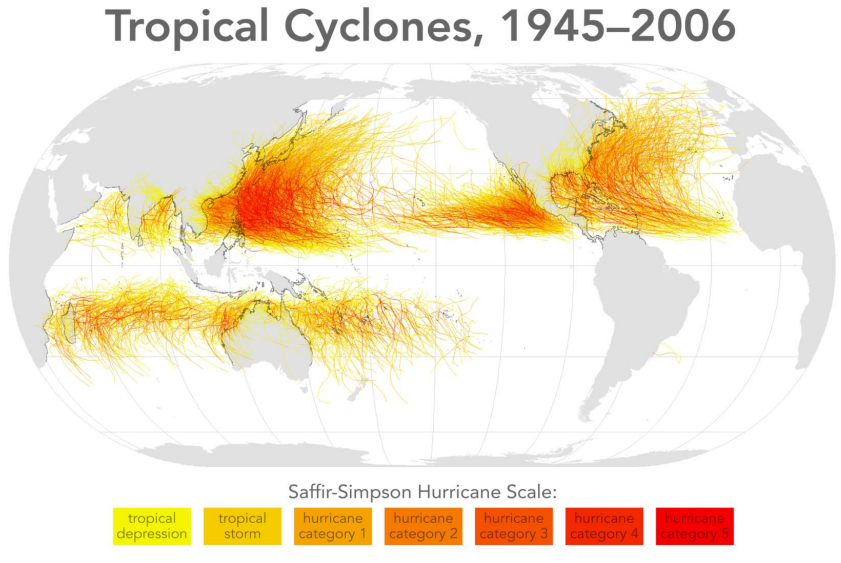
\includegraphics[width=\linewidth]{assets/list.png}
        \captionof{figure}{Path taken by hurricanes and their intensity, 1945-2006, from \cite{swic}}
        \label{fig:cyclones}
    \end{center}
\end{minipage}


\section{Conditions for genesis}
\begin{figure}
    \centering
    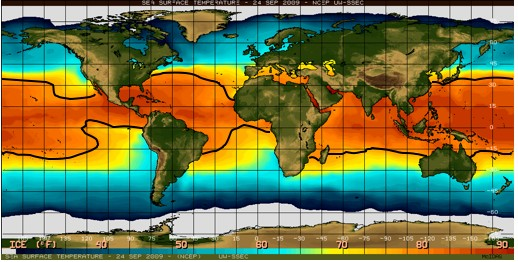
\includegraphics[width=0.7\linewidth]{assets/SSTforGlobalOcean1.jpg}
    \caption{Sea surface temperature around the world. Black lines represent locations where the temperature is sufficiently high enough for hurricane formation (26.5°C)}
    \label{fig:temp}
\end{figure}
As mentioned in the introduction, there are certain conditions that are necessary (but not sufficient) for hurricanes to form. A high-level description of these required conditions are as follow:
\begin{enumerate}
    \item \textit{A sea surface temperature of at least 26.5°C}. Hurricanes take their energy from the heat energy of the ocean through a mix evaporation and latent heat and as such this condition is crucial. For this reason, nearly all hurricanes grow from depressions born within the tropics. Specifically, most hurricanes that hit the east coast of the U.S. are born near the west coast of northern Africa, and grow as they are pushed westward by streams, as seen in figure \ref{fig:temp}. \cite{develop}
    \item \textit{The proper temperature gradient in height} in order to support thunderstorm activity. \cite{develop}
    \item \textit{Sufficient water vapor} in the middle of the troposphere. Often, the middle of the troposphere contains dry air which inhibits the formation of tropical depressions, which are what spawn hurricanes. \cite{develop}
    \item \textit{Sufficient distance from the equator}. As mentioned in the above section on fluid mechanics in a rotated frame: the effects of conservation of angular momentum on hurricane vorticity depend on the Coriolis parameter, which increases as latitude goes away from the equator. Typically, the Coriolis Force becomes significant at about 483km above and below the equator. Outside of these bounds, cyclonic rotation becomes difficult to generate. \cite{develop}
    \item \textit{Little vertical wind shear} from the surface towards the atmosphere. Wind shears inhibit the formation of hurricane and while it is not fully understood why, some research shows that this my be tied to point 3, as it would drag dry air in the middle of the troposphere.
\end{enumerate}


\section{Governing equations of mature hurricanes}

A common way of approaching hurricane modeling is to assume axial symmetry. To take advantage of this, as described in \cite{holton_hakim_2019}, let us put Eqns. \ref{eqn:mom1} and \ref{eqn:mom2} in vector form:

\begin{equation}
    \frac{D\vec{V}}{Dt}+f\vec{k}\times\vec{V}=-\frac{1}{\rho}\vec{\nabla}p
\end{equation}

for the horizontal velocity $\vec{V}=u\hat{\i}+v\hat{\j}$, or alternately we can write the right hand side in terms of the geopotential $\Phi=gh$ using the hydrostatic equation \ref{eqn:hydrobal}:

\begin{equation}
    \frac{D\vec{V}}{Dt}+f\vec{k}\times\vec{V}=-\vec{\nabla}\Phi|_{p=const}
    \label{eqn:momvec}
\end{equation}

% Natural coordinates consist of  $\vec{t}$, the unit vector tangential to the horizontal velocity at any point, $\vec{n}$, the unit vector normal to the horizontal velocity and to the left of the flow direction, and $\vec{k}$, the unit vector pointing directly upward. We can therefore write the horizontal velocity as $\vec{V}=V\vec{t}$, and its material derivative as 
% \begin{equation*}
%     \frac{D\vec{V}}{Dt}=\frac{D(V\vec{t})}{Dt}=\vec{t}\frac{DV}{Dt}+V\frac{D\vec{t}}{Dt}
% \end{equation*}

% \vspace{5mm}
% \begin{minipage}{0.49\textwidth}
%     \vspace{-2ex}
%     \begin{center}
%         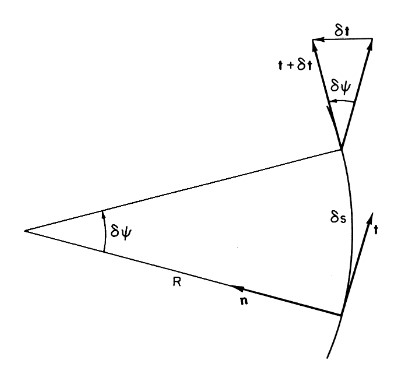
\includegraphics[width=0.7\linewidth]{assets/tangentvector.jpg}
%         \captionof{figure}{Rate of change of the tangent vector to the horizontal flow \cite{holton_hakim_2019}.}
%         \label{fig:tangentvector}
%     \end{center}
% \end{minipage}\hspace{0.05\textwidth}
% \begin{minipage}{0.49\textwidth}
% To find $\frac{D\vec{t}}{Dt}$, consider Fig. \ref{fig:tangentvector}. We can see that
% \begin{equation*}
%     \delta\psi=\frac{\delta s}{R}=\frac{|\delta\vec{t}|}{\vec{t}}=|\delta\vec{t}|
% \end{equation*}
% since $|\vec{t}|=1$. In the limit $\delta s\rightarrow 0$,$|\delta \vec{t}|$ is parallel with $\vec{n}$, so we get 

% \begin{align*}
%     \frac{D\vec{t}}{Dt}=\frac{D\vec{t}}{Ds}\frac{Ds}{Dt}=\frac{\vec{n}}{R}V \\
%     \frac{D\vec{V}}{Dt}=\vec{t}\frac{DV}{Dt}+\vec{n}\frac{V^2}{R}
% \end{align*}
% \end{minipage}
 
% So then since we can express the pressure gradient term as 

% \begin{equation*}
%     -\vec{\nabla}\Phi|_{p=const}=-(\vec{t}\frac{d\Phi}
% \end{equation*}

% ========this whole section is potentially a dud because i think we only need that vector form. whoops



where the gradient is taken along isobars under our assumption of geostrophic flow, so $p$ is constant. From \ref{eqn:momvec}, we can find that in cylindrical co-ordinates (radial position $\vec{r}$, angular position $\vec{\lambda}$, vertical position $\vec{z}$)

\begin{equation}
    \frac{v_{\lambda}}{r}+fv_{\lambda}=\frac{\partial \Phi}{\partial r}
    \label{eqn:windbalance}
\end{equation}
for tangential velocity $v_{\lambda}$. Under the axisymmetric assumption, we can say that the angular momentum $M=rv_{\lambda}+f\frac{r^2}{2}$ is conserved above the frictional boundary layer \cite{smith_montgomery_2017}. \cite{holton_hakim_2019} states that Eqn. \ref{eqn:windbalance} can therefore be written as 

\begin{equation}
    \frac{M^2}{r^3}-\frac{f^2r}{4}=\frac{\partial\Phi}{\partial r}
    \label{eqn:windbalance_mom}
\end{equation}
To eliminate $\frac{\partial \Phi}{\partial r}$ we can continue to follow \cite{holton_hakim_2019} in taking a quick step over from isobaric coordinates to log-pressure coordinates, i.e. where the vertical coordinate is 

\begin{equation*}
    z^*=-H\ln(p/p_s)
\end{equation*}
for reference pressure $p_s$ and scale height $H=RT_s/g$, where $T_s$ is a global average temperature. We can put the hydrostatic balance equation \ref{eqn:hydrobal} in terms of $\Phi= gz$ using the ideal gas law $p=\rho RT$

\begin{equation*}
    gdz = d\Phi=-\frac{RT}{p}dp=-RTd\ln p
\end{equation*}
so
\begin{equation*}
    \frac{\partial\Phi}{\partial \ln p}=-RT
\end{equation*}
Then finally putting into log-pressure coordinates:
\begin{equation*}
    \frac{\partial \Phi}{\partial z^*}=\frac{RT}{H}
\end{equation*}

We can now differentiate our relation in Eqn. \ref{eqn:windbalance_mom} with respect to $z^*$ to get a relationship between the radial temperature gradient in the hurricane and the vertical shear of the angular momentum:

\begin{equation}
    \frac{1}{r^3}\frac{\partial M^2}{\partial z^*}=\frac{R}{H}\frac{\partial T}{\partial r}
    \label{eqn:verticalshear}
\end{equation}

%===include temperature fluctuation bit?

\subsection{The effects of vertical wind shear}

The relationship between the radial temperature gradient and the vertical shear of the angular momentum in Eqn. \ref{eqn:verticalshear} is interesting for numerous reasons, but principally because the vertical wind shear has an impact on the structure of the hurricane vortex \cite{smith_montgomery_2017}.

For instance, vertical wind shear can cause wave-like motion \cite{reasormontgomery2015} that couples with the convection of the hurricane \cite{reimer2013}, causing eddy terms in the equations of motion. It can also tilt the vortex axis from the vertical \cite{Jones1995} and introduce new pathways for dryer air to enter the vortex and reduce instability \cite{reimer2013}. 

As mentioned above, the dynamics of hurricanes are complex, and efforts to model and predict them are just as complex and varied. However, for smaller aspects, we can apply simpler models. Let us consider a model of uniform vertical shear flow in pressure-based coordinates
\begin{equation}
    \bar{U}=U_0+U_z z
\end{equation}

where $U_0$ and $U_z$ are constants, with an axisymmetric barotropic vortex superimposed as described in \cite{Jones1995}. The tangential wind for this system is given by \cite{Jones1995} to be
\begin{equation}
    v_{\lambda} = v_0\frac{s(1+\frac{5b}{2a}s^4)}{(1+as^2+bs^6)^2}
\end{equation}
where $s$ is the ratio of the radius $r$ to the radius of maximum winds $r_{max}=100$ km and $v_0$, $a$, and $b$ are constants. We have the constants for three different runs from \cite{Jones1995} in Table \ref{tab:constants}.

\begin{table}[]
    \centering
    \begin{tabular}{|c|c|c|c|}
    \hline
         Profile&$v_0$&a&b  \\
         \hline
         Standard&71.521&0.3398&$5.377\times10^{-4}$ \\ 
         \hline
         30 m/s &53.641&0.3398&$5.377\times10^{-4}$ \\ 
         \hline
         20 m/s &35.761&0.3398&$5.377\times10^{-4}$ \\ 
         \hline
    \end{tabular}
    \caption{}
    \label{tab:constants}
\end{table}

Recalling from above that $M=rv_{\lambda}+f\frac{r^2}{2}$, we can investigate the relationship between the vertical wind shear and temperature, and model temperature profiles for hurricanes of this model. Substituting the definition for angular momentum into Eqn. \ref{eqn:verticalshear} and applying chain rule gives us 
\begin{equation}
    \frac{1}{r^3}\frac{\partial r}{\partial z^*}\frac{\partial }{\partial r}(rv_{\lambda}(r)+f\frac{r^2}{2})=\frac{R}{H}\frac{\partial T}{\partial r}
\end{equation}
or
\begin{equation}
    \frac{1}{r^3}\frac{\partial r}{\partial z^*}(v_{\lambda}(r)+r\frac{\partial v_{\lambda}}{\partial r}+fr)=\frac{R}{H}\frac{\partial T}{\partial r}
\end{equation}
We clearly need a relation between $r$ and $z^*$ to know anything about $T$. Let's choose the relation between $r$ and $p$ found by \cite{Silvia2001} for the Mexican Pacific Ocean $p=3.8256r+828.7300$. Given that
\begin{equation*}
    p=p_a e^{-z^*/H}
\end{equation*}
we can choose $p_a=101.325 $ kPa and $T_s=13.9$ °C to get
\begin{equation*}
    r=26486.04e^{-z^*/243.28}-216.63
\end{equation*}
or
\begin{equation*}
    \frac{dr}{dz^*}=-108.87e^{-z^*/243.28}
\end{equation*}

Let's choose $z^*=0$ for this exercise. So we have 
\begin{equation*}
    \frac{\partial T}{\partial r} = \frac{36.32}{r^3}(v_{\lambda}(r)+r\frac{\partial v_{\lambda}}{\partial r}+fr)
\end{equation*}
We can integrate this numerically. Let us assume that given we're using a relation from the Mexican Pacific Ocean that our latitude is 20 °N, so $f=2\Omega \sin\theta=4.99\times10^{-5}$ s$^{-1}$. We can then get a temperature profile for radii from 0.1 km to $r_{max}=100$ km, as shown in Fig. \ref{fig:Tplot}.

\begin{figure}
    \centering
    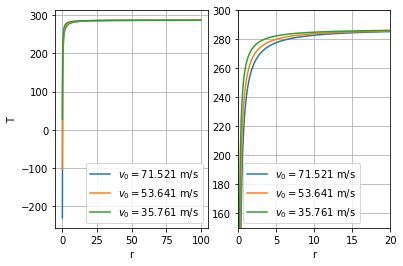
\includegraphics[width=\linewidth]{assets/Tplot.png}
    \caption{The temperature profile with respect to radius. The second plot here is a subset of the first, to see more clearly the differences between different runs.}
    \label{fig:Tplot}
\end{figure}

We see that, for an isobar of pressure $p=p_a$ (given that we took a constant $z^*=0$) the temperature is non-physical for small radii and then approaches the average global temperature as it increases. This is expected, as we know that in the center of a hurricane is the eye, and the dynamics of convection work much differently. Therefore this simple model is not expected to produce physical results for smaller radii. Then, moving outward in the hurricane, the storm decreases in intensity, so it makes sense for the temperatures to approach that of the outside. 

If we chose a larger pressure than the atmospheric pressure, we can see from our equations that we would expect the temperature to be scaled down, and vice versa for smaller pressures. 